% -*- mode: latex; -*-
\documentclass[sigconf]{acmart}

%%
%% \BibTeX command to typeset BibTeX logo in the docs
\AtBeginDocument{%
  \providecommand\BibTeX{{%
    \normalfont B\kern-0.5em{\scshape i\kern-0.25em b}\kern-0.8em\TeX}}}

%% Rights management information.  This information is sent to you
%% when you complete the rights form.  These commands have SAMPLE
%% values in them; it is your responsibility as an author to replace
%% the commands and values with those provided to you when you
%% complete the rights form.
\setcopyright{acmcopyright}
\copyrightyear{2021}
\acmYear{2021}


%%%%%%%%%%%%%%%%%%%%%%%%%%%%%% Packages %%%%%%%%%%%%%%%%%%%%%%%%%%%%%%%%%%%%%%%%
%%%%%%%%%%%%%%%%%%%%%%%%%%%%%%% Packages %%%%%%%%%%%%%%%%%%%%%%%%%%%%%%%%%%%%%%%
\usepackage{graphicx}
\usepackage{epsfig}
\usepackage{times}
\usepackage[ruled,vlined]{algorithm2e}            %% for algorithms
\usepackage{amsmath}
\usepackage{amsthm}                  %% for theorems and definitions
% \usepackage{amssymb}                 %% for arrows like rightarrowtail
\usepackage{amsfonts}                %% \mathbb
\usepackage{mathtools}               %% for coloneqq and others
\usepackage{cases}                   %% better math brackets
\usepackage{mathpartir}              %%% for inference rules
\usepackage[nolist]{acronym}
\usepackage{hyperref}                %% for auto references
\usepackage{xpunctuate}              %% for punctuation's after macros
% \usepackage{cite}                    %% for bibliography ranges
\usepackage{subcaption}              %% For complex figures with subfigures/subcaptions
\usepackage{wrapfig}                 %% wrapping figures around text
\usepackage{listings}                %% for source code lstlisting
\usepackage{enumitem}                %% For better enumerate environment
\setlist[description]{leftmargin=\parindent,labelindent=\parindent}
\usepackage{caption}
\usepackage{multirow}                %% for multiple rows in tables
\usepackage{tikz}                    %% assertion stack visualization
\usepackage[T1]{fontenc}             %% For escaping special characters in bibtex
\usetikzlibrary{matrix}
\usetikzlibrary{arrows}
\usetikzlibrary{positioning}
\usetikzlibrary{shapes.multipart}
\usetikzlibrary{automata}
\usetikzlibrary{cd}                  %% for commuting diagrams

\usepackage{lib/paperCommands}

%%%%%%%%%%%%%%%%%%%%%%%%%%%%%%% End Packages %%%%%%%%%%%%%%%%%%%%%%%%%%%%%%%%%%


%%%%%%%%%%%%%%%%%%%%%%%%%%%%%%% Packages Configs %%%%%%%%%%%%%%%%%%%%%%%%%%%%%%%%%%
\graphicspath{ {./Figures/} }
\raggedbottom

\theoremstyle{definition}
\newtheorem{theorem}{Theorem}[section]
\newtheorem{definition}{Definition}[section]
\newtheorem{corollary}{Corollary}[theorem]
\newtheorem{lemma}[theorem]{Lemma}
\newtheorem*{analysis}{Analysis}

\DeclareMathOperator*{\minimize}{minimize}

\SetKwInOut{Input}{Input}                % Set the Input
\SetKwInOut{Output}{Output}              % set the Output

\lstdefinelanguage{SMTLIB}{
    alsoletter={\-},
    morekeywords={push,pop,assert,check-sat,declare,const,define,fun,and,or,not,check,sat,get,model,reset},
    morecomment=[l]{;},
    morestring=[b]{"},
    sensitive=false,
}

\lstset{
  frame=top,frame=bottom,
  basicstyle=\linespread{.99}\small\normalfont\sffamily,    % the size of the fonts that are used for the code
  commentstyle=\color{Gray},
  keywordstyle=\color{NavyBlue},
  stepnumber=1,                           % the step between two line-numbers. If it is 1 each line will be numbered
  numbersep=10pt,                         % how far the line-numbers are from the code
  tabsize=2,                              % tab size in blank spaces
  extendedchars=true,                     %
  breaklines=true,                        % sets automatic line breaking
  captionpos=t,                           % sets the caption-position to top
  mathescape=true,
  showstringspaces=false,
  escapeinside={(*@}{@*)},%
  literate = {-}{-}1
 }

\newcommand{\lstvdots}{%
  \raisebox{-1pt}[0pt][0pt]{%
    \scalebox{0.7}{\ensuremath{\vdots}}}%
  \hspace{-1.5pt}}

\reversemarginpar
%%%% new environment for sub-proofs
\newenvironment{subproof}[1][\proofname]{%
  \renewcommand{\qedsymbol}{\ensuremath{\blacksquare}}%
  \begin{proof}[#1]%
}{%
  \end{proof}%
}

\newenvironment{MAlgorithm}[1][htb]
  {\renewcommand{\algorithmcfname}{M}% Update algorithm name
   \begin{algorithm}[#1]%
  }{\end{algorithm}}

\renewcommand{\sectionautorefname}{Section }
%%%%%%%%%%%%%%%%%%%%%%%%%%%%%%% End Packages Configs %%%%%%%%%%%%%%%%%%%%%%%%%%%%%%



%%%%%%%%%%%%%%%%%%%%%%%%%%%%%% Kick Off %%%%%%%%%%%%%%%%%%%%%%%%%%%%%%%%%%%%%%%%
\begin{document}

\title{Inspectable Incrementality in Minimum Feedback Arc Set Solving}

\author{Colin Shea-Blymyer}
\email{sheablyc@oregonstate.edu}
\affiliation{%
  \institution{Oregon State University}
  \city{Corvallis}
  \state{Oregon}
  \country{USA}
}
\author{Jeffrey M. Young}
\email{youngjef@oregonstate.edu}
\affiliation{%
  \institution{Oregon State University}
  \city{Corvallis}
  \state{Oregon}
  \country{USA}
}

\renewcommand{\shortauthors}{Shea-Blymyer and Young.}

%%
%% The abstract is a short summary of the work to be presented in the
%% article.
\begin{abstract}
  Abstract here


%%% Local Variables:
%%% mode: latex
%%% TeX-master: "../main"
%%% End:
\end{abstract}

%%
%% Keywords. The author(s) should pick words that accurately describe
%% the work being presented. Separate the keywords with commas.
\keywords{datasets, neural networks, gaze detection, text tagging}

\begin{teaserfigure}
  \begin{subfigure}[t]{0.5\textwidth}
    \centering
    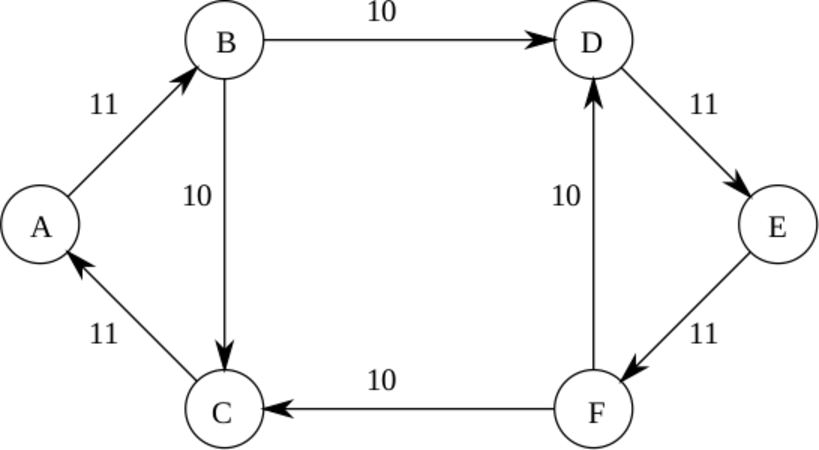
\includegraphics[width=0.80\textwidth]{anti-greed_graph}
    \caption{A three cycle graph which demonstrates that greedily selecting the
      minimum weighted edge will not provide the minimum feedback arc set.}%
    \label{fig:three-cycle}
  \end{subfigure}%
  \hfill
  \begin{subfigure}[t]{0.5\textwidth}
    \centering
    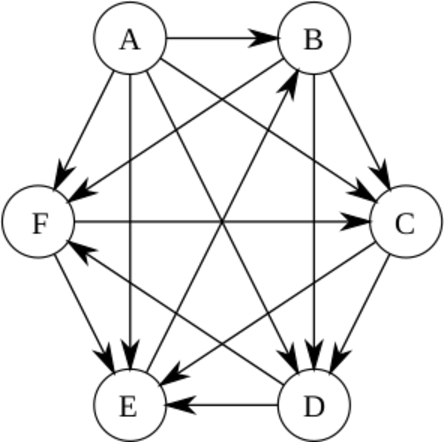
\includegraphics[width=0.45\textwidth]{round_robin_graph}
    \caption{A four cycle graph where each cycle depends on the edge \edge{E}{B}.}
    \label{fig:tournament-graph}
  \end{subfigure}
\end{teaserfigure}

%% information and builds the first part of the formatted document.
\maketitle
%%%%%%%%%%%%%%%%%%%%%%%%%%%%%%% Acronyms %%%%%%%%%%%%%%%%%%%%%%%%%%%%%%%%%%%%%%%
\begin{acronym}[]
  \acro{bcnf}[BCNF]{Boyce---Codd Normal Form}
  \acro{fd}[FD]{functional dependency}
  \acro{3nf}[3NF]{third normal form}
  \acro{cnf}[CNF]{conjunctive normal form}
  \acro{lhs}[lhs]{left hand side}
  \acro{rhs}[rhs]{right hand side}
  % \acro{dsl}[DSL]{domain specific language}
  % \acro{bdd}[BDD]{Binary Decision Diagram}
  \acro{sat}[SAT]{satisfiability solving}
  \acro{smt}[SMT]{satisfiability-modulo theories}
  % \acro{spl}[SPL]{software product-lines}
  % \acro{cdcl}[CDCL]{conflict-driven clause learning}
  \acro{tm}[TM]{Turing Machine}
  \acro{cfg}[CFG]{context-free grammar}
\end{acronym}


\section{Introduction}
\label{section:introduction}%

The minimum feedback arc set problem is a canonical NP-Complete problem given by
\citet{KarpNPComplete}. Worse still, \citet{kannthesis} showed that the problem
is APX-hard. Despite these results finding the minimum feedback arc set of a
directed graph is desirable for many domains: such as certain rank-choice voting
systems, tournament ranking systems\todo{colin citation?}, and dependency graphs
in general.

Solutions to the minimum feedback arc set problem are commonly implemented in
widely used graph libraries yet all suffer from a distinct flaw. While each
implementation provides a solution, the implementations only do so without
allowing the user to inspect intermediate steps; which might contain useful
domain information. For example, the graph \autoref{fig:tournament-graph}
displays a directed graph which encodes a single win tournament system. Each
vertex is a player and each edge encodes a win over a contestant, for example we
see that player E beat contestant B. Observe that the
\autoref{fig:tournament-graph} contains cycles which implies that there is not a
linear ordering amongst the contestants of the tournament, and so any ranking of
the contestants would violate a win of one contestant over another. Removing the
minimum feedback arc set would remove the cycles, which yields a linear order in
the tournament that violates the fewest number of wins. In this example,
intermediate results are edges which compose the minimum feedback arc set, thus
if one had access to the intermediate results one might choose to rematch the
opponents rather than remove the win. Crucially, the result of the rematch may
change the final minimum feedback arc set. Such a procedure could therefore
increase the confidence in the results of the tournament.

To allow for \emph{inspectable incrementality} we propose a novel direction in
solving the minimum feedback arc set problem based on recent advances in
\ac{sat} and \ac{smt} solving. Our approach is to utilize an \ac{smt} solver to
detect cycles and minimize the weight of the feedback arc set. Incrementality in
this approach is given through use of an \emph{incremental} \ac{smt} solver and
generation of \emph{unsatisfiable cores}. A minimum unsatisfiable core is the
minimum set of clauses in a \ac{sat} or \ac{smt} formula which prevent a
\ac{sat} or \ac{smt} solver run from finding a satisfiable assignment. An
incremental solver provides the user the ability to add or remove constraints
and thereby direct the solver during runtime. Incrementality in our approach is
crucial as it allows the user decision points to interact with the solution
process. Thus, a user might observe a unsatisfiable core which corresponds to a
cycle and deliberately resample \emph{only} the edges in the discovered cycle.

Unfortunately, we find that incremental \ac{smt} for finding a minimum feedback
arc set suffers from significant issues which seem to be intractable. In
addition to this result we make the following contributions:
%
\begin{enumerate}
\item An identification of the most intractable problems for an incremental
  \ac{smt} encoding on the minimum feedback arc set problem.
  (\autoref{section:incremental})
\item An \ac{smt} encoding to find the minimum feedback arc set of an arbitrary
  directed and cyclic graph. (\autoref{section:gadgets})
\item An empirical evaluation of the \ac{smt} encoding.
  (\autoref{section:results-and-discussion})
\end{enumerate}



%%% Local Variables:
%%% mode: latex
%%% TeX-master: "../main"
%%% End:
%
\section{Background and Related Work}
\label{section:background}
%
\begin{figure}[h]
  \begin{subfigure}[t]{.45\textwidth}
    \tikzstyle{block} = [draw,fill=blue!20,minimum size=2em, node distance=1cm]
% diameter of semicircle used to indicate that two lines are not connected
\def\radius{.7mm}
\tikzstyle{branch}=[fill,shape=circle,minimum size=3pt,inner sep=0pt]

\begin{tikzpicture}[>=latex']

        % blocks
        \node[block] at (2,-1) (prod) {$SAT$};
        \node[block, name=stging, below=1.0cm of prod] {$SAT$};
        \node[block, name=devel, below=1.0cm of stging] {$SAT$};

        % input nodes
        \node[left of = devel, xshift=-10pt] (input1) {\rV{}};
        \node[left of = stging, xshift=-10pt] (input2) {\qV{}};
        \node[left of = prod, xshift=-10pt] (input3) {\pV{}};

        % inputs
        \draw[->] (input3) -- (prod);
        \draw[->] (input2) -- (stging);
        \draw[->] (input1) -- (devel);

        % outputs
        \draw[->] (prod.east) -- +(1.0,0);
        \draw[->] (stging.east) -- +(1.0,0);
        \draw[->] (devel.east) -- +(1.0,0);


        % \node at (3.5,-3) (result1) {$result$};
        \node[right of = stging, xshift=38pt] (input2) {$result_{\qV{}}$};
        \node[right of = devel, xshift=38pt] (input2) {$result_{\rV{}}$};
        \node[right of = prod, xshift=38pt] (input3) {$result_{\pV{}}$};
\end{tikzpicture}
    \vspace{1.2em}
    \caption{Brute force procedure, no reuse between solver calls.}%
    \label{fig:bkg:bf}
  \end{subfigure}%
  \hfill
  \begin{subfigure}[t]{.45\textwidth}
    \tikzstyle{block} = [draw,fill=blue!20,node distance = 3.2cm, minimum size=2em]

% diameter of semicircle used to indicate that two lines are not connected
\tikzstyle{branch}=[fill,shape=circle,minimum size=3pt,inner sep=0pt]

\begin{tikzpicture}[>=latex']

    % Draw blocks, inputs and outputs

    % \foreach \y in {1,2,3,4,5} {
        % blocks
        \node[block] at (2,-1) (prod) {$SAT$};
        \node[block, name=stging, below=2.75cm of prod] {$SAT$};
        \node[block, name=devel, below=1.0cm of stging] {$SAT$};

        % input nodes
        % \node[left of = devel, xshift=-15pt] (input1) {$development$};
        % \node[left of = stging] (input2) {$\turnBlue{staging}$};
        \node[left of =prod,xshift=-10pt] (input3) {\pV{}};

        % inputs
        \draw[->] (input3) -- (prod);
        \draw[->] (prod) -- node[xshift = 50pt, align=left] {%
          $ \begin{aligned}
            \texttt{pop}  &\quad \eV{}\\
            \texttt{pop}  &\quad \cV{}\\
            \texttt{pop}  &\quad \bV{}\\
            \texttt{push} &\quad (\bV{} \vee \neg \iV{})  \\
            \texttt{push} &\quad \cV{} \\
            \texttt{push} &\quad (\gV{} \rightarrow \cV{}) \\
          \end{aligned}
          $
        } (stging);
\draw[->] (stging) -- node[xshift = 70pt, align=left] {%
  $\begin{aligned}
    & \texttt{resetAssertionStack}\\
    &\texttt{push} \quad \zV{} \leftrightarrow (a \wedge b \wedge c \wedge e)
    % \text{pop} &\quad \kf{pti} \rightarrow c_{i.1}\\
    % \text{pop} &\quad (\kf{spectre\_v2} \vee \kf{l1tf}) \leftrightarrow \\&\quad (c_{0} \wedge (\kf{nospec\_store\_bypass\text{-}disable} \rightarrow f_{j})\\
    % \text{pop} &\quad (c_{0.0} \wedge c_{1} \wedge \ldots c_{n})\\
  \end{aligned}
  $
} (devel);

        % outputs
        \draw[->] (prod.east) -- +(1.0,0);
        \draw[->] (stging.east) -- +(1.0,0);
        \draw[->] (devel.east) -- +(1.0,0);


        % \node at (3.5,-3) (result1) {$result$};
        % \node[right of = stging, xshift=15pt] (input2) {$result$};
        % \node[right of = devel, xshift=15pt] (input2) {$result$};
        % \node at (3.5,-1) (input3) {$result$};

        \node[right of = stging, xshift=38pt] (input2) {$result_{\qV{}}$};
        \node[right of = devel, xshift=38pt] (input2) {$result_{\rV{}}$};
        \node[xshift=19pt] at (3.8,-1) (input3) {$result_{\pV{}}$};
    % }
    % \node[block] at (2,-6) (block6) {$f_6$};
    % \draw[->] (block6.east) -- +(0.5,0);

    % % Calculate branch point coordinate
    % \path (input1) -- coordinate (branch) (block1);

    % % Define a style for shifting a coordinate upwards
    % % Note the curly brackets around the coordinate.
    % \tikzstyle{s}=[shift={(0mm,\radius)}]
    % % It would be natural to use the yshift or xshift option, but that does
    % % not seem to work when shifting coordinates.

    % \draw[->] (branch) node[branch] {}{ % draw branch junction
    %         \foreach \c in {2,3,4,5} {
    %             % Draw semicircle junction to indicate that the lines are
    %             % not connected. The intersection between the lines are
    %             % calculated using the convenient -| syntax. Since we want
    %             % the semicircle to have its center where the lines intersect,
    %             % we have to shift the intersection coordinate using the 's'
    %             % style to account for this.
    %             [shift only] -- ([s]input\c -| branch) arc(90:-90:\radius)
    %             % Note the use of the [shift only] option. It is not necessary,
    %             % but I have used it to ensure that the semicircles have the
    %             % same size regardless of scaling.
    %         }
    %     } |- (block6);
\end{tikzpicture}
    \caption{Incremental procedure, reuse defined by \rn{pop} and \rn{push}.}%
      % sat calls share state that is determined by }
    \label{fig:bkg:inc}
  \end{subfigure}
  \caption{Comparison of incremental and non-incremental \ac{sat} procedures.}%
  \label{fig:bkg}
\end{figure}
%

In this section, we provide background on the minimum feedback arc set problem,
incremental \ac{sat} and \ac{smt} solving, and unsatisfiable cores. We begin
with preliminaries on graphs and feedback arc sets. We close the section with a
description of incremental \ac{sat} solving and \ac{smt} solving.

On a directed graph \graph{G}{V}{E} a \emph{feedback arc set} \fas{S} is a set
of edges in $\kf{E}$, such that removing them from the graph $\kf{G}$ results in
an acyclic graph. The minimum feedback arc set problem finds the
\optimal{\fas{S}} of the minimum size. For weighted graphs, one might desire
\optimal{\fas{S}} to have the minimum total weight of any \fas{S}. Finding this
\optimal{\fas{S}} is the minimum weighted feedback arc set problem.

%
%
With the minimum feedback arc set problem defined, we provide the following
background on incremental \ac{sat} solvers and assume knowledge of \ac{smt}
solvers. Suppose, we have three related propositional formulas that we desire to
solve.
%
\begin{align*}
  p &=\ a \wedge b \wedge c \wedge e  \\
  q &=\ a \wedge (b \vee \neg \iV{}) \wedge c \wedge (\gV{} \rightarrow c) \\
  r &=~z \leftrightarrow (a \wedge b \wedge c \wedge e)
\end{align*}
%
\pV{} is simply a conjunction of variables. In \qV{}, relative to \pV{}, we see
that the variables \iV{} and \gV{} are added, \eV{} is removed, and there are
two new clauses: $(b \vee \neg \iV{})$ and $(\gV{} \rightarrow c)$, both of
which possibly affect the values of \bV{} and \cV{}. In \rV{}, the variables and
constraints introduced in \pV{} are further constrained to a new variable,
\zV{}.

Suppose one wants to find a model for each formula. Using a non-incremental
\ac{sat} solver results in the procedure illustrated in \autoref{fig:bkg:bf};
where \ac{sat} solving is a batch process and no information is reused.
Alternatively, a procedure using an incremental \ac{sat} solver is illustrated
in \autoref{fig:bkg:inc}; in this scenario, all formulas are solved by single
solver instance where terms are programmatically added or removed from the
solver.

The ability to add and remove terms is enabled by manipulating the
\textit{assertion stack}, to add or remove levels on the stack. The incremental
interface provides two commands: \rn{push} to create a new \emph{scope} and add
a level to the stack, and \rn{pop} to remove the topmost level on the stack.
Consider the following \acl{smtlib} program which demonstrates three levels on
the assertion stack. The \acl{smtlib} standard~\cite{BarFT-SMTLIB} is an
international standard that defines a general interface for \ac{sat} and
\ac{smt} solvers. The program follows the procedure outlined in
\autoref{fig:bkg:inc} and solves \pV, \qV{} and \rV{}:

\begin{lstlisting}[columns=flexible,keepspaces=true,language=SMTLIB]
(declare-const a Bool)         ;; variable declarations for p
(declare-const b Bool)
(declare-const c Bool)
(declare-const e Bool)
(assert a)                     ;; a is shared between p and q
(push)                         ;; solve p
  (assert e)
  (assert c)
  (assert b)
  (check-sat)                  ;; check-sat on p
(pop)                          ;; remove e, c, and b assertions
(push)                         ;; solve for q
  (declare-const i Bool)       ;; new variables
  (declare-const g Bool)
  (assert (or b (not i)))      ;; new clause
  (assert c)                   ;; re-add c
  (assert (=> g c))            ;; new clause
  (check-sat)                  ;; check sat of q
(pop)                          ;; i and g out of scope
(reset)                        ;; reset the assertion stack
(declare-const a Bool)         ;; variable declarations for r
(declare-const b Bool)
(declare-const c Bool)
(declare-const e Bool)
(declare-const z Bool)
(assert (= z (and a (and b (and c (and e ))))))
(check-sat)                    ;; check-sat on r
\end{lstlisting}

We begin by defining \pV{}, and assert $\kf{a}$ outside of a new scope so that
it can be reused for \qV{}. Internally, all levels on the assertions stack are
conjoined and asserted when a \rn{check-sat} command is issued. Thus, we reuse
$a$ by exploiting this conjunction behavior. Had we asserted
\lstinline{(and a (and b (and c (and e))))}, then we would not be able to reuse
only the assertion on $a$ since it was created in conjunction with other
variables. The first \rn{push} command enters a new level on the assertion
stack, the remaining variables are asserted and we issue a \rn{check-sat} call.
After the \rn{pop} command, all assertions and declarations from the previous
level are removed. Thus, after we solve \qV{} the variables $i$ and $g$ cannot
be referenced as they are no longer in scope. Similarly, after the first
\rn{check-sat} call and subsequent \rn{pop}, \eV{}, \cV{} and \bV{} are no
longer defined.

In an efficient process one would initially add as many \emph{shared} terms as
possible, such as $a$ from \pV{} and then reuse that term as many times as
needed. An efficient process should perform only enough manipulation of the
assertion stack as required to reach the next \ac{sat} problem of interest from
the current one. However, notice that doing so is not entirely straight forward;
we were only able to reuse $a$ from \pV{} in \qV{} because we defined \pV{} in a
non-intuitive way by utilizing the internal behavior of the assertion stack.
This situation is exacerbated by \ac{sat} problems such as \rV{}, where due to
the equivalence between a new term and shared terms, we are forced to completely
remove everything on the stack with a \rn{reset} command just to construct
\rV{}. Thus incremental \ac{sat} solvers provide the primitive operations
required to solve related \ac{sat} problems efficiently, yet writing the
\acl{smtlib} program to solve the set efficiently is not straightforward.

%%% Local Variables:
%%% mode: latex
%%% TeX-master: "../main"
%%% End:
%
\section{Approach and SAT Encoding}
\label{section:gadgets}

Dem ga\textbf{gd}ets



%%% Local Variables:
%%% mode: latex
%%% TeX-master: "../main"
%%% End:
%
\section{Case Studies}
\label{section:case-studies}

To evaluate this approach, we construct a prototype \ac{smt}-enabled algorithm
and assess the prototype on Erd\H{o}s-R\'{e}nyi graphs. Erd\H{o}s-R\'{e}nyi
graphs are generated according to two parameters: $\kf{p}$, a metric of
connectedness for the graph, and $\kf{k}$ is the number of vertices in the
graph. In addition, we add a parameter $\kf{s}$ which represents the size of the
range of possible weights on edges in a graph.

With these parameters we employ random generation to construct sample graphs. We
are interested in the individual effect $\kf{k}$, $\kf{p}$ and $\kf{s}$ have on
runtime, in addition to the interactions effects between each parameter.
Consider the case where $\kf{p}$ and $\kf{k}$ are left unbound, yet $\kf{s}$ is
set to 1. This is the specific case where solving the minimum weighted feedback
arc set problem solves the minimum feedback arc set problem. Thus, by setting
$\kf{s}$ to 1 we generate graphs to solve the minimum feedback arc set problem.
Consider the case where $\kf{s}$ is larger than one. In this case, edges must
possess positive weights and the weighted minimum feedback arc set may be
different than the minimum feedback arc set.

\NOTE{Hi Mike. The rest of the section is describing each case individually and
  then research questions. We don't have these spelled out right now. What we
  hypothesize is that at some combination of $\kf{k}$, $\kf{p}$ and $\kf{s}$ the
solver runtime will become infeasible. Then we can make determinations on the
viability of this method in different domains. For example, most tournaments
will be a bounded number of participants, and score ranges, but may have maximum
connectivity. Thus, we would be able to make a conclusion on the viability of
our method for the tournament domain.}



%%% Local Variables:
%%% mode: latex
%%% TeX-master: "../main"
%%% End:
%
\section{Results and Discussion}
\label{section:results-and-discussion}

It was good enough to graduate



%%% Local Variables:
%%% mode: latex
%%% TeX-master: "../main"
%%% End:


\bibliographystyle{ACM-Reference-Format}
\bibliography{bib/paper}


%% If your work has an appendix, this is the place to put it.
\appendix
\section{Appendix}%
\label{appendix:source-code-listings}
Source code listings

\begin{lstlisting}[language=python]
  """- Module    : app.py
  - Copyright : (c) Jeffrey M. Young
  ; (c) Colin Shea-Blymyer
  - License   : BSD3
  - Maintainer: youngjef@oregonstate.edu, sheablyc@oregonstate.edu
  - Stability : experimental

  """

  from pprint     import pprint
  from functools  import reduce
  import z3       as z
  import igraph   as ig
  import numpy    as np

  import matplotlib.pyplot as plt
  import timeit
  from tqdm import tqdm

  import graphs  as gs
  import utils   as u

def MFAS_set_cover(s,graph):
    """Find the minimum feedback arc set by encoding it as a minimum set cover.
    The encoding requires a cycle matrix which we find externally to the SAT
    solver. Then given the cycle matrix we do the following encoding:

    Variables:
      - m is |E|
      - w_{j} is the weight of edge j \in E (we don't implement the weight matrix)
      - y_{j} is a symbolic edge; y_{j} = 1 if edge j is in the feedback edge set and 0 otherwise
      - a is the cycle matrix
      - a_{ij} is the value of edge j in cycle i; a_{ij} = 1 if j participates, 0 otherwise


    minimize(sum{j = 1}^{m}(w_{j} * y_{j}))

      subject to:

    sum_{j = 1}^{m}(a_{ij} * y_{j}) >= 1
    \forall i. y_{i} \in {0,1}
    """

    ## initialization
    m            = graph.ecount()
    cycle_matrix = u.mk_cycle_matrix(u.find_all_cycles(graph), m)
    n, c         = graph.get_adjacency().shape
    num_cycles   = len(cycle_matrix)
    edge_list    = graph.get_edgelist()
    sym_to_edge_cache = {}
    edge_to_sym_cache = {}
    sum_var      = 'y'


    def symbolize(i,j):
        "given two indices, create a symbolic variable"
        new = z.Int('{0}->{1}'.format(i,j))
        return new


    def constraint_1(i,s_edge):
        """ Multiply the edge by its corresponding value in the cycle matrix
        """
        edge  = sym_to_edge_cache[s_edge]
        value = 0
        if edge in cycle_matrix[i]:
            value = cycle_matrix[i][edge]

        return (value * s_edge)


    ## symbolize the edges
    for source,sink in edge_list:
            s_edge                           = symbolize(source, sink)
            ## an edge is either a 0 or a 1
            s.add(z.Or([s_edge == 0, s_edge == 1]))

            sym_to_edge_cache[s_edge]        = (source,sink)
            edge_to_sym_cache[(source,sink)] = s_edge


    ## Perform constraint 1 and add it to the solver instance
    for i in range(num_cycles):
        s.add(z.Sum([constraint_1(i,s_edge)
                     for s_edge in sym_to_edge_cache.keys()]) >= 1)


    ## we want the smallest y possible
    s.minimize(z.Sum([s_edge for s_edge in sym_to_edge_cache.keys()]))

    s.check()
    return s.model()
\end{lstlisting}


\newpage
\begin{lstlisting}[language=python]
  def runWithGraph(graph):
  s = z.Optimize()
  return MFAS_set_cover(s, graph), u.get_feedback_arc_set(graph)


  def runErdosRenyi(n,p):
  """Given n vertices and a probability, p of edges. Find the minimum
  feedback arc set of an erdos-renyi graph

  """
  s = z.Optimize()
  g = ig.Graph.Erdos_Renyi(n, p, directed=True, loops=True)
  while g.is_dag():
  g = ig.Graph.Erdos_Renyi(n, p, directed=True, loops=True)

  return MFAS_set_cover(s,g), u.get_feedback_arc_set(g)

  def runWattsStrogatz(dim, size, nei, p):
  """Given the dimension of the lattice, size of the lattice along all
  dimensions, the number of steps within which two vertices are connected
  (nei), and the probability p, find the minimum feedback arc set of a
  watts-strogatz graph

  """
  s = z.Optimize()
  g = ig.Graph.Watts_Strogatz(dim, size, nei, p, loops=True, multiple=False)
  while g.is_dag():
  g = ig.Graph.Watts_Strogatz(dim, size, nei, p, loops=True, multiple=False)

  return MFAS_set_cover(s,g), u.get_feedback_arc_set(g)
\end{lstlisting}

\newpage
\begin{lstlisting}[language=python]
"""
- Module    : utils.py
- Copyright : (c) Jeffrey M. Young
            ; (c) Colin Shea-Blymyer
- License   : BSD3
- Maintainer: youngjef@oregonstate.edu, sheablyc@oregonstate.edu
- Stability : experimental

Common utility functions
"""

from z3 import *
import networkx as nx
from numpy import empty
from re import split

def make_name(frm,to): return frm + "->" + to

def parse_edge(edge): # return list(map(int,edge.__str__().split("->")))
    str_edge = edge.__str__()
    inner    = list(map(lambda x: x, str_edge.split("->")))
    return tuple(map(lambda x : int(x), inner))

def parse_core(core):
    """Parse an unsat core. An unsat core is shallowly embedded as a list of z3
    BoolRef objects such as: [1->2, 2->3, 3->4, 4->1], to operate on these we
    need to coerce them to a string parse the string and coerce the Ints out.

    Input:  List of strings, e.g.,      [1->2  , 2->3  , 3->4  , 4->1  ]
    Output: List of List of Ints, e.g., [[1, 2], [2, 3], [3, 4], [4, 1]]

    """
    return list(map(lambda e: parse_edge(e), core))

def edge_to_list_dict(g):
    """ Convert a graph to a dictionary of edges
    """
    ret = {}
    for source,sink in g.get_edgelist():
        if source not in ret.keys():
            ret[source] = []

        ret[source].append(sink)

    return ret

def remove_edge(g,source,sink):
    """Given an igraph graph, a source vertex and a sink vertex remove the edge
    connecting the source and the sink from the igraph graph. This function
    mutates g.
    """
    g.delete_edges(g.get_eid(source,sink))


def flatten(list_o_lists):
    return [e for sublist in list_o_lists for e in sublist]


def find_all_cycles(graph):
    nx_graph = graph.to_networkx()
    return list(nx.simple_cycles(nx_graph))


def pairs(ls, n = 1):
    return list(zip(ls, ls[n:] + ls[:n]))


def mk_cycle_matrix(cycle_edge_list, num_edges):
    ps          = [pairs(edges) for edges in cycle_edge_list]
    cycle_count = len(cycle_edge_list)
    matrix      = []
    for i in range(cycle_count):
        cycle = {}
        for pair in ps[i]:
            cycle[pair] = 1

        matrix.append(cycle)

    return matrix

def get_feedback_arc_set(graph):
    fas = graph.feedback_arc_set(method="ip")
    return list(map(lambda x : graph.es[x].tuple, fas))
\end{lstlisting}




\end{document}
\endinput
